% Options for packages loaded elsewhere
\PassOptionsToPackage{unicode}{hyperref}
\PassOptionsToPackage{hyphens}{url}
%
\documentclass[
  8pt,
  ignorenonframetext,
]{beamer}
\usepackage{pgfpages}
\setbeamertemplate{caption}[numbered]
\setbeamertemplate{caption label separator}{: }
\setbeamercolor{caption name}{fg=normal text.fg}
\beamertemplatenavigationsymbolsempty
% Prevent slide breaks in the middle of a paragraph
\widowpenalties 1 10000
\raggedbottom
\setbeamertemplate{part page}{
  \centering
  \begin{beamercolorbox}[sep=16pt,center]{part title}
    \usebeamerfont{part title}\insertpart\par
  \end{beamercolorbox}
}
\setbeamertemplate{section page}{
  \centering
  \begin{beamercolorbox}[sep=12pt,center]{part title}
    \usebeamerfont{section title}\insertsection\par
  \end{beamercolorbox}
}
\setbeamertemplate{subsection page}{
  \centering
  \begin{beamercolorbox}[sep=8pt,center]{part title}
    \usebeamerfont{subsection title}\insertsubsection\par
  \end{beamercolorbox}
}
\AtBeginPart{
  \frame{\partpage}
}
\AtBeginSection{
  \ifbibliography
  \else
    \frame{\sectionpage}
  \fi
}
\AtBeginSubsection{
  \frame{\subsectionpage}
}
\usepackage{amsmath,amssymb}
\usepackage{lmodern}
\usepackage{iftex}
\ifPDFTeX
  \usepackage[T1]{fontenc}
  \usepackage[utf8]{inputenc}
  \usepackage{textcomp} % provide euro and other symbols
\else % if luatex or xetex
  \usepackage{unicode-math}
  \defaultfontfeatures{Scale=MatchLowercase}
  \defaultfontfeatures[\rmfamily]{Ligatures=TeX,Scale=1}
\fi
% Use upquote if available, for straight quotes in verbatim environments
\IfFileExists{upquote.sty}{\usepackage{upquote}}{}
\IfFileExists{microtype.sty}{% use microtype if available
  \usepackage[]{microtype}
  \UseMicrotypeSet[protrusion]{basicmath} % disable protrusion for tt fonts
}{}
\makeatletter
\@ifundefined{KOMAClassName}{% if non-KOMA class
  \IfFileExists{parskip.sty}{%
    \usepackage{parskip}
  }{% else
    \setlength{\parindent}{0pt}
    \setlength{\parskip}{6pt plus 2pt minus 1pt}}
}{% if KOMA class
  \KOMAoptions{parskip=half}}
\makeatother
\usepackage{xcolor}
\newif\ifbibliography
\setlength{\emergencystretch}{3em} % prevent overfull lines
\providecommand{\tightlist}{%
  \setlength{\itemsep}{0pt}\setlength{\parskip}{0pt}}
\setcounter{secnumdepth}{-\maxdimen} % remove section numbering
% type setting
% ------------------------------------------------------------------------------
\usepackage[german]{babel}     

% fonts
% ------------------------------------------------------------------------------
\usefonttheme{professionalfonts}

% slide title and horizontal line
% ------------------------------------------------------------------------------
\setbeamertemplate{frametitle}{%
    \vskip-30pt \color{black}\large%
    \begin{minipage}[b][23pt]{120mm}%
    \flushleft\insertframetitle%
    \end{minipage}%
}

\setbeamertemplate{headline}										
{
\vskip10pt\hfill\hspace{3.5mm} 										 
\vskip15pt\color{black}\rule{\textwidth}{0.4pt} 					 
}

% slide number
% ---------------------------------------------------------------
\setbeamertemplate{navigation symbols}{}
\setbeamertemplate{footline}
{
\vskip5pt
\vskip2pt
\makebox[123mm]{\hspace{7.5mm}
\hfill Wahrscheinlichkeitstheorie und Frequentistische Inferenz $\vert$ 
\copyright $ $ 2023 Dirk Ostwald CC BY-NC-SA 4.0 $\vert$ 
Folie \insertframenumber}
\vskip4pt
}

% block color scheme
% ------------------------------------------------------------------------------
% colors
\definecolor{white}{RGB}{255,255,255}
\definecolor{grey}{RGB}{235,235,235}
\definecolor{lightgrey}{RGB}{245,245,245}
\definecolor{LightBlue}{RGB}{220,220,255}
\definecolor{darkblue}{RGB}{51, 51, 153}

% definitions and theorems
\setbeamercolor{block title}{fg = black, bg = grey}
\setbeamercolor{block body}{fg = black, bg = lightgrey}

% general line spacing 
% ------------------------------------------------------------------------------
\linespread{1.3}

% local line spacing
% ------------------------------------------------------------------------------
\usepackage{setspace}

% colors
% -----------------------------------------------------------------------------
\usepackage{color}

% justified text
% ------------------------------------------------------------------------------
\usepackage{ragged2e}
\usepackage{etoolbox}
\apptocmd{\frame}{}{\justifying}{}

% bullet point lists
% -----------------------------------------------------------------------------
\setbeamertemplate{itemize item}[circle]
\setbeamertemplate{itemize subitem}[circle]
\setbeamertemplate{itemize subsubitem}[circle]
\setbeamercolor{itemize item}{fg = black}
\setbeamercolor{itemize subitem}{fg = black}
\setbeamercolor{itemize subsubitem}{fg = black}
\setbeamercolor{enumerate item}{fg = black}
\setbeamercolor{enumerate subitem}{fg = black}
\setbeamercolor{enumerate subsubitem}{fg = black}
\setbeamerfont{itemize/enumerate body}{}
\setbeamerfont{itemize/enumerate subbody}{size = \normalsize}
\setbeamerfont{itemize/enumerate subsubbody}{size = \normalsize}

% color links
% ------------------------------------------------------------------------------
\usepackage{hyperref}
\definecolor{urls}{RGB}{204,0,0}
\hypersetup{colorlinks, citecolor = darkblue, urlcolor = urls}


% additional math commands
% ------------------------------------------------------------------------------
\usepackage{bm}                                         % bold math symbols
\newcommand{\niton}{\not\owns}

% text highlighting
% ------------------------------------------------------------------------------
\usepackage{soul}
\makeatletter
\let\HL\hl
\renewcommand\hl{%
  \let\set@color\beamerorig@set@color
  \let\reset@color\beamerorig@reset@color
  \HL}
\makeatother

% equation highlighting
% -----------------------------------------------------------------------------
\newcommand{\highlight}[2][yellow]{\mathchoice%
  {\colorbox{#1}{$\displaystyle#2$}}%
  {\colorbox{#1}{$\textstyle#2$}}%
  {\colorbox{#1}{$\scriptstyle#2$}}%
  {\colorbox{#1}{$\scriptscriptstyle#2$}}}%

% additional mathematical operators
% ------------------------------------------------------------------------------
\DeclareMathOperator*{\argmax}{arg\,max}
\DeclareMathOperator*{\argmin}{arg\,min}

\ifLuaTeX
  \usepackage{selnolig}  % disable illegal ligatures
\fi
\IfFileExists{bookmark.sty}{\usepackage{bookmark}}{\usepackage{hyperref}}
\IfFileExists{xurl.sty}{\usepackage{xurl}}{} % add URL line breaks if available
\urlstyle{same} % disable monospaced font for URLs
\hypersetup{
  hidelinks,
  pdfcreator={LaTeX via pandoc}}

\author{}
\date{\vspace{-2.5em}}

\begin{document}

\begin{frame}[plain]{}
\protect\hypertarget{section}{}
\center

\begin{center}\includegraphics[width=0.2\linewidth]{1_Abbildungen/wtfi_1_otto} \end{center}

\vspace{2mm}

\Large

Wahrscheinlichkeitstheorie und Frequentistische Inferenz \vspace{6mm}

BSc Psychologie WiSe 2022/23

\vspace{6mm}

Prof.~Dr.~Dirk Ostwald
\end{frame}

\begin{frame}[plain]{}
\protect\hypertarget{section-1}{}
\vfill
\center
\Huge

\textcolor{red}{Aufnahme läuft!} \vfill
\end{frame}

\begin{frame}[plain]{}
\protect\hypertarget{section-2}{}
\vfill
\center
\huge

\textcolor{black}{(1) Einführung} \vfill
\end{frame}

\begin{frame}[plain]{}
\protect\hypertarget{section-3}{}
\vfill
\begin{large}
Prof. Dr. Dirk Ostwald (dirk.ostwald@ovgu.de)
\end{large}
\vspace{.7cm}

\begin{minipage}{.3\linewidth}
\begin{center}
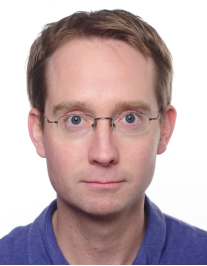
\includegraphics[scale=.6]{1_Abbildungen/wtfi_1_dirk.pdf}
\end{center}
\end{minipage}
\begin{minipage}{.7\linewidth}
\begin{small}
\renewcommand{\arraystretch}{1.3}
\begin{tabular}{ll}
Seit 2021   & W2 Professur Methodenlehre I              \\
2014 - 2020 & W1 Professur Freie Universität Berlin     \\
2010 - 2014 & Postdoc BCCN \& MPIB Berlin               \\
2007 - 2010 & PhD Psychologie Birmingham                \\
2004 - 2006 & MSc Neurowissenschaften Tübingen          \\
2005 - 2012 & BSc Mathematik Hagen                      \\
2000 - 2003 & BSc Medizin Hamburg                       \\
\end{tabular}
\end{small}
\end{minipage}
\vspace{.7cm}

\begin{large}
\begin{tabular}{ll}
Forschung   & Komputationale Kognitive Neurowissenschaften  \\
Lehre       & Datenwissenschaft
\end{tabular}
\end{large}
\vfill
\end{frame}

\begin{frame}{}
\protect\hypertarget{section-4}{}
\href{https://www.ipsy.ovgu.de/methodenlehre_I-path-980,1404.html}{\textcolor{darkblue}{Homepage}}

\begin{center}\includegraphics[width=0.7\linewidth]{1_Abbildungen/wtfi_1_homepage} \end{center}
\end{frame}

\begin{frame}{}
\protect\hypertarget{section-5}{}
\vfill
\setstretch{2.3}
\Large

Datenwissenschaft und Statistik

Formalia

Studium und Diskussion

Selbstkontrollfragen
\end{frame}

\begin{frame}{}
\protect\hypertarget{section-6}{}
\vfill
\setstretch{2.3}
\Large

\textbf{Datenwissenschaft und Statistik}

Formalia

Studium und Diskussion

Selbstkontrollfragen
\end{frame}

\begin{frame}{Datenwissenschaft und Statistik}
\protect\hypertarget{datenwissenschaft-und-statistik}{}
\vfill

\center
\huge

\textcolor{darkblue}{Datenwissenschaft} \vspace{5mm}

\Large

Die Kunst, aus Daten Sinn zu generieren
\end{frame}

\begin{frame}{Datenwissenschaft und Statistik}
\protect\hypertarget{datenwissenschaft-und-statistik-1}{}
\vspace{2mm}

\begin{center}\includegraphics[width=0.9\linewidth]{1_Abbildungen/wtfi_1_datenwissenschaft_komponenten} \end{center}
\vfill
\end{frame}

\begin{frame}{Datenwissenschaft und Statistik}
\protect\hypertarget{datenwissenschaft-und-statistik-2}{}
\Large

Datenwissenschaft ist Datenreduktion

\center
\vspace{.4cm}

\begin{center}\includegraphics[width=0.8\linewidth]{1_Abbildungen/wtfi_1_datenreduktion} \end{center}
\end{frame}

\begin{frame}{Datenwissenschaft und Statistik}
\protect\hypertarget{datenwissenschaft-und-statistik-3}{}
\Large

Datenwissenschaft ist Naturwissenschaft \vspace{3mm}

\begin{center}\includegraphics[width=1\linewidth]{1_Abbildungen/wtfi_1_wissenschaft} \end{center}
\end{frame}

\begin{frame}{Datenwissenschaft und Statistik}
\protect\hypertarget{datenwissenschaft-und-statistik-4}{}
\Large

Datenwissenchaft ist Dateninterpretation \center \vspace{.5cm}

\begin{center}\includegraphics[width=0.8\linewidth]{1_Abbildungen/wtfi_1_datenwissenschaftslinse} \end{center}
\end{frame}

\begin{frame}{Datenwissenschaft und Statistik}
\protect\hypertarget{datenwissenschaft-und-statistik-5}{}
\Large

Terminologie der Datenwissenschaft \vspace{.5cm}

\center

Statistik = Maschinelles Lernen = Künstliche Intelligenz \vspace{.5cm}

\small
\renewcommand{\arraystretch}{1.5}
\begin{tabular}{l|l|l}

Statistik                   & Maschinelles Lernen       & Künstliche Intelligenz        \\\hline
Probabilistische Modelle    & Deterministische Modelle  & Agenten-basierte Modelle      \\
Theoretische Analyse        & Klassifikation            & Reinforcement learning        \\
Optimalitätstheorie         & Bayesianische Modelle     & Symbolik                      \\
Asymptotische Theorie       & Anwendung                 & Anwendung                     \\
Wissenschaftsphilosophie    & Benchmarking              & Hype                          \\
\end{tabular}
\end{frame}

\begin{frame}{Datenwissenschaft und Statistik}
\protect\hypertarget{datenwissenschaft-und-statistik-6}{}
\vfill

\center
\huge

\textcolor{darkblue}{Datenwissenschaft in der Psychologie} \vspace{5mm}

\Large

Die Kunst, aus Verhaltens- und Neurophysiologiedaten

psychologischen Sinn zu generieren
\end{frame}

\begin{frame}{Datenwissenschaft und Statistik}
\protect\hypertarget{datenwissenschaft-und-statistik-7}{}
\center
\huge

\textcolor{darkblue}{Statistik} \vspace{5mm}

\Large

Die Kunst, aus Daten Sinn zu generieren

\textbf{und seine assoziierte Unsicherheit zu quantifizieren}
\end{frame}

\begin{frame}{Datenwissenschaft und Statistik}
\protect\hypertarget{datenwissenschaft-und-statistik-8}{}
\begin{center}\includegraphics[width=1\linewidth]{1_Abbildungen/wtfi_1_statistik_themen} \end{center}
\end{frame}

\begin{frame}{Datenwissenschaft und Statistik}
\protect\hypertarget{datenwissenschaft-und-statistik-9}{}
\vspace{.5cm}

\begin{minipage}{.6\linewidth}
\center

\begin{center}\includegraphics[width=0.8\linewidth]{1_Abbildungen/wtfi_1_statistik_geschichte} \end{center}

\end{minipage}
\hspace{.5cm}
\begin{minipage}{.1\linewidth}
\center

\begin{center}\includegraphics[width=3\linewidth]{1_Abbildungen/wtfi_1_efron_buch} \end{center}

\end{minipage}
\end{frame}

\begin{frame}{Datenwissenschaft und Statistik}
\protect\hypertarget{datenwissenschaft-und-statistik-10}{}
\center
\huge

\textcolor{darkblue}{Statistik in der Psychologie}

\vspace{5mm}
\Large

Die Kunst, aus Verhaltens- und Neurophysiologiedaten

psychologischen Sinn zu generieren

\textbf{und seine assoziierte Unsicherheit zu quantifizieren}
\end{frame}

\begin{frame}{Datenwissenschaft und Statistik}
\protect\hypertarget{datenwissenschaft-und-statistik-11}{}
\vfill
\setstretch{1.7}

\textcolor{darkblue}{Klassische Partition der Statistik in der Psychologie}

\begin{itemize}
\tightlist
\item
  Deskriptivstatistik
\item
  Inferenzstatistik
\item
  Multivariate Statistik
\end{itemize}

\textcolor{darkblue}{Sinnvolle Partition der psychologischen Datenwissenschaft}

\begin{itemize}
\tightlist
\item
  Wahrscheinlichkeitstheoretische Grundlagen
\item
  Frequentistische Inferenz
\item
  Allgemeines Lineares Modell
\item
  Bayesianische Inferenz
\item
  Multivariate Datenanalyse
\end{itemize}

\vfill
\end{frame}

\begin{frame}{Datenwissenschaft und Statistik}
\protect\hypertarget{datenwissenschaft-und-statistik-12}{}
\vfill
\setstretch{3}

\textcolor{darkblue}{Fundamentale Annahmen der Wahrscheinlichkeitstheorie}
\vspace{1mm}

\begin{itemize}
\tightlist
\item
  \justifying  Zufallsprozesse können mathematisch modelliert werden.
\item
  Mathematik kann zur Vorhersage zufälliger Ereignisse genutzt werden.
\item
  Die Wahrscheinlichkeitstheorie ist mengentheoretisch begründet.
\end{itemize}
\end{frame}

\begin{frame}{Datenwissenschaft und Statistik}
\protect\hypertarget{datenwissenschaft-und-statistik-13}{}
\textcolor{darkblue}{Fundamentale Annahmen der Frequentistischen Inferenz}
\vspace{1mm}

\begin{itemize}
\item
  \justifying Wahrscheinlichkeiten spiegeln die relative Frequenz des
  Auftretens eines zufälligen Ereignisses und beschreiben objektive
  Eigenschaften der realen Welt. \vspace{1mm}
\item
  Die Parameter probabilistischer Modelle sind feste, unbekannte
  Konstanten, die als \emph{wahre, aber unbekannte, Parameterwerte}
  bezeichnet werden. Über Parameterwerte und Modelle werden keine
  probabilistischen Aussagen getroffen. \vspace{1mm}
\item
  Statistische Methoden werden so gestaltet, dass sie gute langfristige
  relative Frequenzeigenschaften besitzen und werden typischerweise
  anhand ihrer Stichprobenverteilungen bewertet.
\end{itemize}
\end{frame}

\begin{frame}{Datenwissenschaft und Statistik}
\protect\hypertarget{datenwissenschaft-und-statistik-14}{}
\textcolor{darkblue}{Fundamentale Annahmen der Bayesianischen Inferenz}
\vspace{1mm}

\begin{itemize}
\item
  \justifying Wahrscheinlichkeiten werden als Grade der Sicherheit,
  nicht als langfristige relative Häufigkeiten interpretiert. Aussagen
  der Form ``Die Wahrscheinlichkeit, dass das Wintersemester 2022/23
  vollständig in Präsenzlehre stattfindet, ist 0.9.'' haben eine
  Bedeutung. \vspace{1mm}
\item
  Die Parameter probabilistischer Modelle sind feste, unbekannte
  Konstanten, die als \emph{wahre, aber unbekannte, Parameterwerte}
  bezeichnet werden. Über Parameterwerte und Modelle werden
  probabilistische Aussagen getroffen, die unseren Grad an Sicherheit
  hinsichtlich ihrer quantitativen Ausprägung und Validität
  widerspiegeln. \vspace{1mm}
\item
  Probabilistische Aussagen über Parameter werden mithilfe von
  Wahrscheinlichkeitsverteilungen getroffen, auf deren Grundlage
  optimale Entscheidungen im Sinne von Kosten-Nutzenfunktionen getroffen
  werden können.
\end{itemize}
\end{frame}

\begin{frame}{Datenwissenschaft und Statistik}
\protect\hypertarget{datenwissenschaft-und-statistik-15}{}
\textcolor{darkblue}{Datenwissenschaftliches Curriculum der OVGU Psychologie}

\setstretch{1.5}

\begin{itemize}
\tightlist
\item
  Mathematische Grundlagen

  \begin{itemize}
  \tightlist
  \item
    Mengen, Funktionen, Differentialrechnung, Integralrechnung, \ldots{}
  \end{itemize}
\item
  Wahrscheinlichkeitstheorie

  \begin{itemize}
  \tightlist
  \item
    Maßtheoretische Grundlagen, Zufallsvariablen, Erwarungswert,
    Varianz, \ldots{}
  \end{itemize}
\item
  Frequentistische Inferenz

  \begin{itemize}
  \tightlist
  \item
    Statistische Modelle, Schätztheorie, Konfidenzintervalle,
    Hypothesentesten,\ldots{}
  \end{itemize}
\item
  Allgemeines Lineares Modell

  \begin{itemize}
  \tightlist
  \item
    Matrizen, multivariate Normalverteilung, Schätztheorie,
    Studiendesigns, \ldots{}
  \end{itemize}
\item
  Bayesianische Inferenhz

  \begin{itemize}
  \tightlist
  \item
    Konjugierte Modelle, numerische Inferenz, variational inference,
    \ldots{}
  \end{itemize}
\item
  Multivariate Methoden

  \begin{itemize}
  \tightlist
  \item
    Multivariates ALM, Faktoranalyse, Neuronale Netze, \ldots{}\\
  \end{itemize}
\item
  Programmierung

  \begin{itemize}
  \tightlist
  \item
    Grundlagen von R, Python, Matlab, Linux, Parallel computing,
    \ldots{}
  \end{itemize}
\end{itemize}
\end{frame}

\begin{frame}{Formalia}
\protect\hypertarget{formalia}{}
\textcolor{darkblue}{Modul B1 Deskriptive Statistik | Wahrscheinlichkeitstheorie und Frequentistische Inferenz}
\setstretch{2}

\begin{itemize}
\tightlist
\item
  \justifying Donnerstags 13-16 Uhr in Raum G40B-231
\item
  Kursmaterialien (Folien, Videos, RMarkdown Code) auf der
  \href{https://bit.ly/3yT42Sj}{\textcolor{darkblue}{Kurswebseite}}
\item
  Code auf
  \href{https://github.com/dirk-ostwald/wahrscheinlichkeitstheorie-und-frequentistische-inferenz-23}{\textcolor{darkblue}{Github}}
\item
  Ankündigungen über die
  \href{https://elearning.ovgu.de/course/view.php?id=13805}{\textcolor{darkblue}{Moodleseite}}
\item
  Empfohlene Lektüre ist
  \href{https://wasd.urz.uni-magdeburg.de/dostwald/}{\textcolor{darkblue}{PDWP}}
\item
  \href{https://bit.ly/3qJKlan}{\textcolor{darkblue}{Link zu vorheriger Iteration des Kurses}}
\item
  \href{https://bit.ly/3SNh3nR}{\textcolor{darkblue}{Link zum Kurs Mathematische Grundlagen}}
\item
  Tutorium Mittwochs 11-13 Uhr mit Belinda Fleischmann
\end{itemize}
\end{frame}

\begin{frame}[t]{Formalia}
\protect\hypertarget{formalia-1}{}
\vspace{1mm}

\textcolor{darkblue}{Modul B1 Deskriptive Statistik | Wahrscheinlichkeitstheorie und Frequentistische Inferenz}
\vspace{1mm}

\small
\center
\footnotesize
\renewcommand{\arraystretch}{1.1}
\begin{tabular}{lll}
Datum        & Einheit                       & Thema                                             \\\hline
13.10.2021   & Einführung                    & (1) Einführung                                    \\
20.10.2021   & Wahrscheinlichkeitstheorie    & (2) Wahrscheinlichkeitsräume                      \\
27.10.2021   & Wahrscheinlichkeitstheorie    & (3) Zufallsvariablen                              \\
03.11.2021   & Wahrscheinlichkeitstheorie    & (4) Zufallsvektoren                               \\
10.11.2021   & Wahrscheinlichkeitstheorie    & (5) Erwartungswert und Kovarianz                  \\
17.11.2021   & Wahrscheinlichkeitstheorie    & (6) Ungleichungen und Grenzwerte                  \\
24.11.2021   & Wahrscheinlichkeitstheorie    & (7) Normalverteilungstransformationen             \\
01.12.2021   & Frequentistische Inferenz     & (8) Statistische Modelle, Statistiken, Schätzer   \\
08.12.2021   & Frequentistische Inferenz     & (9) Schätzereigenschaften                         \\
15.12.2021   & Frequentistische Inferenz     & (10) Konfidenzintervalle                          \\
             & \textcolor{gray}{Weihnachtspause}                                                 \\
05.01.2022   & Frequentistische Inferenz     & (11) Hypothesentests                              \\
12.01.2022   & Frequentistische Inferenz     & (12) T-Tests                                      \\
19.01.2022   & Frequentistische Inferenz     & (13) Einfaktorielle Varianzanalyse                \\
26.01.2022   & Frequentistische Inferenz     & (14) Zweifaktorielle Varianzanalyse               \\\hline
Feb 2022     & Klausurtermin                 &                                                   \\
Jul 2022     & Klausurwiederholungstermin    &
\end{tabular}
\end{frame}

\begin{frame}{Formalia}
\protect\hypertarget{formalia-2}{}
\textcolor{darkblue}{Modul B1 Deskriptive Statistik | Wahrscheinlichkeitstheorie und Frequentistische Inferenz}
\setstretch{2.5}

\begin{itemize}
\tightlist
\item
  Vorlesungsfolien inklusive Selbstkontrollfragen sind klausurrelevant
\item
  Altklausuren finden sich auf den Kurswebseiten früherer Jahre
\item
  Benotete Multiple Choice Klausur (30 Fragen) Ende Wintersemester
  2022/23
\item
  Klausurwiederholungstermin am Ende des Sommersemesters 2023
\item
  Klausurtermin und Klausurort gemäß Prüfungsplan des
  \href{https://www.fnw.ovgu.de/Studium/Pr\%C3\%BCfungsamt.html}{\textcolor{darkblue}{FNW Prüfungsamtes}}
\end{itemize}
\end{frame}

\begin{frame}{}
\protect\hypertarget{section-7}{}
\vfill
\setstretch{2.3}
\Large

Datenwissenschaft und Statistik

Formalia

\textbf{Studium und Diskussion}

Selbstkontrollfragen
\end{frame}

\begin{frame}{Studium und Diskussion}
\protect\hypertarget{studium-und-diskussion}{}
\large

\href{https://elearning.ovgu.de/mod/feedback/view.php?id=384185}{\textcolor{darkblue}{Umfrage zum Studienstart}}
\end{frame}

\begin{frame}{Studium und Diskussion}
\protect\hypertarget{studium-und-diskussion-1}{}
\setstretch{2.2}
\large

\textcolor{darkblue}{Studium $\neq$ Schule} \normalsize

\begin{itemize}
\tightlist
\item
  Schule ist Pflicht, Studium ist freiwillig.
\item
  Sie wollen nicht studiert werden, Sie wollen studieren.
\item
  Sie sind motiviert.
\item
  Studium ist Arbeit mit 40-Stundenwoche.
\item
  Wir machen keinen Osterhasenunterricht.
\item
  Klausuren dienen Ihnen, nicht den Lehrenden.
\item
  Veranstaltungen dienen der Organisation, nicht des Erwerbs von Wissen.
\end{itemize}
\end{frame}

\begin{frame}{Studium und Diskussion}
\protect\hypertarget{studium-und-diskussion-2}{}
\setstretch{2.2}
\large

\textcolor{darkblue}{Studium $\neq$ Berufsausbildung} \normalsize

\begin{itemize}
\tightlist
\item
  Das Studium dient dem Erwerb theoretischen Wissens.
\item
  Studium = Reproduktion, Praxis = Translation, Wissenschaft =
  Reflexion.
\item
  Sie werden nie wieder so viel Zeit zum Erwerb theoretischen Wissens
  haben.
\item
  Nach Studienabschluss sind Sie keine Psychotherapeut:in.
\item
  Nach Studienabschluss haben sie viel über Psychologie gelesen.
\item
  Praktische Fähigkeiten lernt man in der Praxis, nicht in der Theorie.
\item
  Denken und lernen Sie interdisziplinär, Fachgrenzen sind für Faule.
\end{itemize}
\end{frame}

\begin{frame}{Studium und Diskussion}
\protect\hypertarget{studium-und-diskussion-3}{}
\large
\setstretch{1.2}

\textcolor{darkblue}{Lernphasen} \small

Phase 1: Überblicken

\begin{itemize}
\tightlist
\item
  Überblick durch Vorlesung/Überfliegen der Materialien.
\item
  Verstehen einfacher Zusammenhänge.
\item
  Verstehen, was man nicht versteht.
\end{itemize}

Phase 2: Verstehen

\begin{itemize}
\tightlist
\item
  Erarbeiten des Verstehens komplexer Zusammenhänge.
\item
  Schriftliche Beantwortung der Selbstkontrollfragen.
\item
  Klärung von Details.
\end{itemize}

Phase 3: Memorisieren

\begin{itemize}
\tightlist
\item
  Auswendiglernen aller Inhalte.
\item
  Aktive Wiedergabe der Inhalte, schriftlich oder mündlich.
\item
  Teilnahme an der Klausur.
\end{itemize}

Teilen Sie große Aufgaben immer in viele kleine, gut zu bewältigende
Aufgaben!

Sie machen Schreibtischarbeit, treiben Sie also täglich Sport!
\end{frame}

\begin{frame}{Studium und Diskussion}
\protect\hypertarget{studium-und-diskussion-4}{}
\large

\textcolor{darkblue}{Verschiedenes} \vspace{2mm} \justifying \normalsize

Ist Statistik schwer? \vspace{1mm}

Ich kann kein Mathe, Statistik macht mich fertig. Was soll ich bloß tun?
\vspace{1mm}

Psychotherapeut:in wollte ich eigentlich jetzt erstmal nicht werden,
sondern ich will Menschen verstehen. Wozu brauche ich da Statistik?
\vspace{1mm}

Ich würde gerne verstehen, wie das Gehirn funktioniert. In welchem Kurs
bekomme ich die Antwort? \vspace{1mm}

Warum muss ich etwas über wissenschaftliche Methoden lernen, ich will
doch viel lieber Menschen helfen?
\end{frame}

\begin{frame}{Studium und Diskussion}
\protect\hypertarget{studium-und-diskussion-5}{}
\setstretch{1.1}

\textcolor{darkblue}{Approbationsordnung für Psychotherapeutinnen und Psychotherapeuten (2020)}
\footnotesize \vspace{2mm}

Inhalte, die im Bachelorstudiengang im Rahmen der hochschulischen Lehre
zu vermitteln und bei dem Antrag auf Zulassung zur psychotherapeutischen
Prüfung nachzuweisen sind.

\noindent \textbf{9. wissenschaftliche Methodenlehre}

Die studierenden Personen (\ldots)

\begin{enumerate}
[a)]
\setcounter{enumi}{2}
\item
  wenden Begriffe, Methoden und Ergebnisse der qualitativen und
  quantitativen Forschung in der psychologischen Grundlagen- und
  Anwendungsforschung an,
\item
  beurteilen die Auswirkungen von Forschungsmethoden auf
  Untersuchungspopulationen und wenden deskriptive und
  inferenzstatistische Methoden sowie weitere statistische Verfahren zur
  Auswertung von Ergebnissen grundlagen- und anwendungsbezogener Studien
  in verschiedenen Bereichen der psychologischen und
  psychotherapeutischen Forschung an,
\item
  planen wissenschaftliche Untersuchungen, führen diese Untersuchungen
  durch und werten sie aus, (\ldots)
\end{enumerate}

\textcolor{darkblue}{$\quad\Rightarrow$ Bachelorarbeit}

Zur Vermitllung der Inhalte der wissenschaftlichen Methodenlehre sind
bei der Planung der hochschulischen Lehre (\ldots) die folgenden
Wissensbereiche abzudecken (\ldots)

\begin{enumerate}
[a)]
\setcounter{enumi}{2}
\item
  deskriptive und Inferenz-Statistik (\ldots)
\item
  Datenerhebung und Datenanalyse unter Nutzung digitaler Technologien.
\end{enumerate}
\end{frame}

\begin{frame}{Studium und Diskussion}
\protect\hypertarget{studium-und-diskussion-6}{}
\setstretch{1.1}

\textcolor{darkblue}{Approbationsordnung für Psychotherapeutinnen und Psychotherapeuten (2020)}
\vspace{2mm}

\footnotesize

Inhalte, die im Masterstudiengang im Rahmen der hochschulischen Lehre zu
vermitteln und bei dem Antrag auf Zulassung zur psychotherapeutischen
Prüfung nachzuweisen sind. \vspace{1mm}

\footnotesize

\noindent \textbf{2. vertiefte Forschungsmethodik}

Die studierenden Personen

\begin{enumerate}
[a)]
\item
  wenden komplexe und multivariate Erhebungs- und Auswertungsmethoden
  zur Evaluierung und Qualitätssicherung von Interventionen an,
\item
  nutzen und beurteilen einschlägige Forschungsstudien und deren
  Ergebnisse für die Psychotherapie
\item
  planen selbstständig Studien zur Neu- oder Weiterentwicklung der
  Psychotherapieforschung oder der Forschung in angrenzenden Bereichen,
  führen solche Studien durch, werten sie aus und fassen sie zusammen,
  (\ldots)
\end{enumerate}

\textcolor{darkblue}{$\quad\Rightarrow$ Masterarbeit}

Zur Vermitllung der Inhalte der vertieften Forschnungsmethodik sind bei
der Planung der hochschulischen Lehre (\ldots) die folgenden
Wissensbereiche abzudecken (\ldots)

\begin{enumerate}
[a)]
\tightlist
\item
  multivariate Verfahren und Messtheorie
\end{enumerate}
\end{frame}

\begin{frame}{Studium und Diskussion}
\protect\hypertarget{studium-und-diskussion-7}{}
\Huge
\vfill
\center

Q \& A \vfill
\end{frame}

\begin{frame}{}
\protect\hypertarget{section-8}{}
\vfill
\setstretch{2.3}
\Large

Datenwissenschaft und Statistik

Formalia

Studium und Diskussion

\textbf{Selbstkontrollfragen}
\end{frame}

\begin{frame}{Selbstkontrollfragen}
\protect\hypertarget{selbstkontrollfragen}{}
\setstretch{3}

\begin{enumerate}
\tightlist
\item
  Nennen Sie die drei Hauptkomponenten der Datenwissenschaft.
\item
  Nennen Sie drei Grundannahmen der Wahrscheinlichkeitstheorie.
\item
  Nennen Sie drei Grundannahmen der Frequentistischen Inferenz.
\item
  Nennen Sie drei Grundannahmen der Bayesianischen Inferenz.
\end{enumerate}
\end{frame}

\end{document}
